% DO NOT COMPILE THIS FILE DIRECTLY!
% This is included by the other .tex files.

\begin{frame}[t,plain]
\titlepage
\end{frame}

\begin{frame}[t]{Sources}
\begin{itemize}
\item Presentation available at \url{http://bit.ly/wsn-final}.
\item Based on ideas in Werner-Allen, Geoffrey, Konrad Lorincz, Mario Ruiz, Omar Marcillo, Jeff Johnson, Jonathan Lees, and Matt Welsh. 2006. “Deploying a Wireless Sensor Network on an Active Volcano.” Internet Computing, IEEE 10 (2). IEEE: 18–25.
\begin{itemize}
\item Full text is viewable at \url{http://www.cs.harvard.edu/~mdw/papers/volcano-ieeeic06.pdf}
\end{itemize}
\item Proposal can be found at \url{http://claymcleod.github.io/papers/engr691-final-project/paper.pdf}
\end{itemize}
\end{frame}

\begin{frame}[t,fragile]{Motivation}
\begin{itemize}
\item<1-> Paper discusses authors implementing a wireless sensor network (WSN) to track volcanic activity remotely.
\item<2-> What problems did they encounter?
\begin{itemize}
\item<3-> Gathering accurate data from events \only<5>{\color{red}{X}}
\item<3-> High availability of sensors \only<5>{\color{red}{X}}
\item<3-> Time synchronization across nodes \only<5>{$\checkmark$}
\item<3-> Low radio bandwidth to work with \only<5>{$\checkmark$}
\item<3-> Node failure could impact communication \only<5>{$\checkmark$}
\item<3-> Radio links are lossy and frequently asymmetrical \only<5>{$\checkmark$}
\end{itemize}
\item<4-> \textbf{Summary:}~the solution in my final project aims to alleviate any subproblem related to data collectionand time synchronization, usually by abstracting them away.
\end{itemize}
\end{frame}

\begin{frame}[t,fragile]{Fetch Data Collection}
\begin{itemize}[<+->]
\item \textbf{Goal}: build a reliable data-collection protocol that is used to retrieve buffered data from each node over a multihop network.
\item \textbf{Idea}
\begin{enumerate}
\item The sensor node breaks it’s data down into 256 bytes, then
tags these blocks with timestamps and sequence numbers.
\item The laptop then sends packets out to the target node ID
identifying which sequence numbers it is missing from that
node.
\item In turn, the node will send the missing chunks until the laptop
indicates it has received all sequences.
\item Because the network is sparse, the laptop uses \textbf{flooding} to request data from the network.
\end{enumerate}
\end{itemize}
\end{frame}

\begin{frame}[t,fragile]{Visualization}

\only<2>{A node indicates that an activity has occurred based on some input threshold.}
\only<3>{That node communicates back to the base station, letting it know that an event has been perceived}
\only<4>{When the base station receives enough signal, a data collection is initiated}
\only<5>{Nodes closest to the base station attempt to transfer their data to the base station while the request propigates through the WSN}
\only<6>{Eventually, all nodes are communicating with the base station}
\def\layersep{2.5cm}

\begin{center}
\begin{tikzpicture}[shorten >=1pt,->,draw=black!50, node distance=\layersep]
    \tikzstyle{every pin edge}=[<-,shorten <=1pt]
    \tikzstyle{neuron}=[circle,fill=black!25,minimum size=17pt,inner sep=0pt]
    \tikzstyle{input neuron}=[neuron, fill=blue!50];
    \tikzstyle{output neuron}=[neuron, fill=red!50];
    \tikzstyle{hidden neuron}=[neuron, fill=blue!50];
    \tikzstyle{annot} = [text width=4em, text centered]

    % Draw the input layer nodes
    \foreach \name / \y in {1,...,4}
    % This is the same as writing \foreach \name / \y in {1/1,2/2,3/3,4/4}
        \node[input neuron] (I-\name) at (0,-\y) {};

    % Draw the hidden layer nodes
    \foreach \name / \y in {1,...,5}
        \path[yshift=0.5cm]
            node[hidden neuron] (H-\name) at (\layersep,-\y cm) {};

    % Draw the output layer node
    \node[output neuron, right of=H-3] (O) {};

    % Connect every node in the input layer with every node in the
    % hidden layer.
    \visible<1-4>{
    \foreach \source in {1,...,4}
        \foreach \dest in {1,...,5}
            \path (I-\source) edge (H-\dest);
	}
	
	\visible<1-3>{
    % Connect every node in the hidden layer with the output layer
    \foreach \source in {1,...,5}
        \path (H-\source) edge (O);
    }
    
    \visible<2-3>{\node[input neuron, yellow] (I-3) at (0,-3) {}; }
    \visible<3-3>{\path[yellow, line width=2pt] (I-3) edge (H-3);}
    \visible<3-3>{\path[yellow, line width=2pt] (H-3) edge (O);}
    \only<4>{
    		\foreach \source in {1,...,5}
        		\path[yellow, line width=2pt] (O) edge (H-\source);
    }
    \only<5>{
    		\foreach \source in {1,...,5}
        		\path[green, line width=2pt] (H-\source) edge (O);
        		
        	\foreach \source in {1,...,4}
        		\foreach \dest in {1,...,5}
            		\path[yellow, line width=2pt] (H-\dest) edge (I-\source);
    }
    
    \only<6>{
    		\foreach \source in {1,...,5}
        		\path[green, line width=2pt] (H-\source) edge (O);
        		
        	\foreach \source in {1,...,4}
        		\foreach \dest in {1,...,5}
            		\path[green, line width=2pt] (I-\source) edge (H-\dest);
    }
\end{tikzpicture}
\end{center}
\end{frame}

\begin{frame}[t,fragile]{Experiment}
\begin{itemize}
\item<1-> Designate one node as a \textbf{master} node (connected through serial connection to laptop) and two nodes as \textbf{slave} nodes. 
\begin{itemize}
\item<1-> \textit{Due to the limited number of supplies, only 2 slave nodes can be fabricated}
\end{itemize}
\item<2-> Using a light sensor attached to the circuit board, we can simluate our own event by setting a threshold by how much light is present to trigger an event.
\item<3-> Data about the amount of light present will be constantly recorded and trasmitted to the base station once an event has occurred using the protocol described earlier.
\end{itemize}
\end{frame}

\begin{frame}[t,fragile]{Comparison with Paper}
\begin{center}
\begin{tabular}{| l | l | l | c |}
\hline
Description & Paper & Project & Comparable \\
\hline
Data Type & Seismic Activity & Light Presence & \color{red}{X} \\
Data Frequency & Continuous & Continuous & $\checkmark$ \\
Node Distance & 200-400m & $<$ 10m & \color{red}{X} \\
Network & Lossy & Consistent & \color{red}{X} \\
Hardware & IEEE 802.15.4 & IEEE 802.15.4 & $\checkmark$ \\
Software & TinyOS & TinyOS & $\checkmark$ \\
\hline
\end{tabular}
\end{center}
\end{frame}

\begin{frame}[t,fragile]{Block Storage}
\begin{itemize}
\item<1-> Configuration File
\begin{itemize}
\item<1-> Declare \texttt{BlockStorageC} and hook up to implementation
\end{itemize}
\item<2-> Main File
\begin{itemize}
\item<2-> Explicitly state that the implementation uses \texttt{interface BlockRead} and \texttt{interface BlockWrite}
\item<2-> Implement the following methods on the interface
\begin{itemize}
\item<2-> \texttt{BlockWrite.writeDone}
\item<2-> \texttt{BlockWrite.eraseDone}
\item<2-> \texttt{BlockWrite.syncDone}
\item<2-> \texttt{BlockRead.readDone}
\item<2-> \texttt{BlockRead.computeCrcDone}
\end{itemize}
\end{itemize}
\item<3-> Potentially define interface for storing data
\end{itemize}
\end{frame}

\begin{frame}[t,fragile]{Results}
\vfill
\vspace{1em}
\begin{center}
\pause
{\Large \textit{In Progress (TBD)}}
\end{center}
\vfill
\end{frame}

\begin{frame}[t,fragile]{}
\vfill
\vspace{3em}
\begin{center}
{\Huge Questions?}
\end{center}
\vfill
\end{frame}
